%!TEX root=../main.tex

In recent years, the analysis of multivariate functional data has become a popular method with applications in several fields. Functional principal component analysis (FPCA) is an extension of principal components analysis to functional data. FPCA has become a prevalent tool in FDA due to its abililty to convert infinite-dimensional functional data into finite-dimensional vectors of random scores. Multivariate functional principal components analysis (MFPCA) is the extension of FPCA to multivariate functional data. It allows to identify and visualize the main sources of variation in the data. 

We discuss the estimation of the number of components method in the recently published paper titled ``Multivariate Functional Principal Component Analysis for Data Observed on Different (Dimensional) Domains'' by \cite{happMultivariateFunctionalPrincipal2018a}. For ease of presentation, we use the same notation as theirs.


We briefly present the estimation of MFPCA. For a detailled description of the estimation process, see \cite[Section 3]{happMultivariateFunctionalPrincipal2018a}. In \cite{happMultivariateFunctionalPrincipal2018a}, the authors first estimate the principal components for each individual feature and combine them to derive the multivariate components. So, they chose a number of components for each individual feature and then use only these ones to compute the multivariate components. Let $K_p$ be the number of components retained for the $p$th feature. As the univariate components are concatenated to estimated the multivariate components, the number of multivariate components that can be estimated is $\sum_p K_p$. We however claim that only $\min_p K_p$ can only be accurately estimated.

The estimation of the number of components can also be done using the percentage of variance explained. 

We are interested by the estimation of the eigenvalues of functional datasets. Let $\{\nu_k\}_{1 \leq k \leq K}$ be the set of true eigenvalues and $\{\widehat{\nu}_k\}_{1 \leq k \leq K}$ be the set of estimated eigenfunctions. Simulations are the same as the first setting in \cite{happMultivariateFunctionalPrincipal2018a}. The accuracy of the resulting estimates $\widehat{\nu}_j$ is measured by the relative errors $\text{Err}(\widehat{\nu}_j)  = (\nu_j - \widehat{\nu}_j)^2 / \nu^2_j$. The percentage of variance explained by the $k$th component is defined as
\begin{equation}\label{eq:pve}
     \text{PVE}_k = \frac{\nu_k}{\sum_{k = 1}^K \nu_k}.
\end{equation}
The cumulative percentage of variance explained by the first $k$ components is given by
\begin{equation}\label{eq:cum_pve}
     \text{PVE}_{1:k} = \frac{\sum_{l = 1}^k \nu_l}{\sum_{l^\prime = 1}^K \nu_{l^\prime}}.
\end{equation}
Given a certain percentage of variance explained $\alpha$, the number of components needed to explain at least $\alpha\%$ of the variance of the data is
\begin{equation}\label{eq:npc}
     \text{NPC}_{\alpha} = \sum_{k = 1}^K \mathbf{1}\left\{\text{PVE}_{1:k} < \alpha\right\} + 1 = \min_{k = 1, \dots, K} \text{PVE}_{1:k} > \alpha.
\end{equation}

The simulation setting is based on the simulation in \cite{happMultivariateFunctionalPrincipal2018a}. The data-generating process is based on a truncated version of the Karhunen-Loève decomposition. First, we generate a large orthonormal basis $\{\psi_k\}_{1 \leq k \leq K}$ of $\sLp{\TT{}}$ on an interval $\TT{} = [0, T] \subset \RR$. We fix $T_1 = 0$ and $T_{P + 1} = T$ and we generate $P - 1$ cutting points $T_2, \dots, T_P$ uniformly in $\TT{}$ such that $0 = T_1 < \cdots < T_P < T_{P+1} = T$. Let $s_1, \dots, s_P \in \{-1, 1\}$ be coefficients that randomly flip the eigenfunctions with probability $0.5$. The univariate components of the eigenfunctions are then defined as
\begin{equation}\label{eq:simulation_uni_component}
    \phi_k^{(p)}(t_p) = s_p \restr{\psi_k}{[T_p, T_{p + 1}]}\left(\frac{t_p - T_p}{T_{p + 1} - T_p}\right), \quad k = 1, \dots, K, \quad p = 1, \dots, P.
\end{equation}
The notation $\restr{\phi_k}{[T_p, T_{p + 1}]}$ is the restriction of the function $\phi_k$ to the set $[T_p, T_{p + 1}]$. The set of multivariate functions $\{\psi_k\}_{1 \leq k \leq K}$ is an orthonormal system in $\HH \coloneqq \sLp{\TT{1}} \times \dots \times \sLp{\TT{P}}$ with $\TT{p} = [0, 1]$. Each curve is then simulated using the truncated multivariate Karhunen-Loève expansion:
\begin{equation}
    X(\pointt) = \sum_{k = 1}^K \rho_k \phi_k(\pointt), \quad \pointt \in \TT{},
\end{equation}
where the scores $\rho_k$ are sampled as random normal variables with mean $0$ and variance $\nu_k$. The eigenvalues $\nu_k$ are defined with an exponential decrease, $\nu_k = \exp(-(k + 1)/2)$. We simulate, for each replication of the simulation, $N = 25, 50$ and $100$ observations. Similarly, each component is sampled on a regular grid of $M = 25, 50$ and $100$ sampling points. We compare the methods for $P = 5$ features and we set $K = 50$. The estimation are done using the \textsf{R} package \texttt{MFPCA} \citep{happ-kurzObjectOrientedSoftwareFunctional2020}.

For each univariate feature $p$, we estimate $K_p = 5$ principal components. Then, following the multivariate components estimation procedure, we can estimate $\sum_{p = 1}^P K_p = 25$ multivariate components. The results of the errors of the estimation of the eigenvalues are presented in Figure \ref{fig:ncomp}. We remark that the accuracy of the estimation decreases with the number of components in every scenario. While there is a clear jump in the accuracy for the last five estimated eigenvalues, it seems difficult to set a general rule. \textcolor{red}{...} The number of multivariate eigencomponents that should be estimated is $\min_p K_p$, otherwise the univariate components do not contain enough information to recover accurately their multivariate counterpart.
\begin{figure}
     \centering
    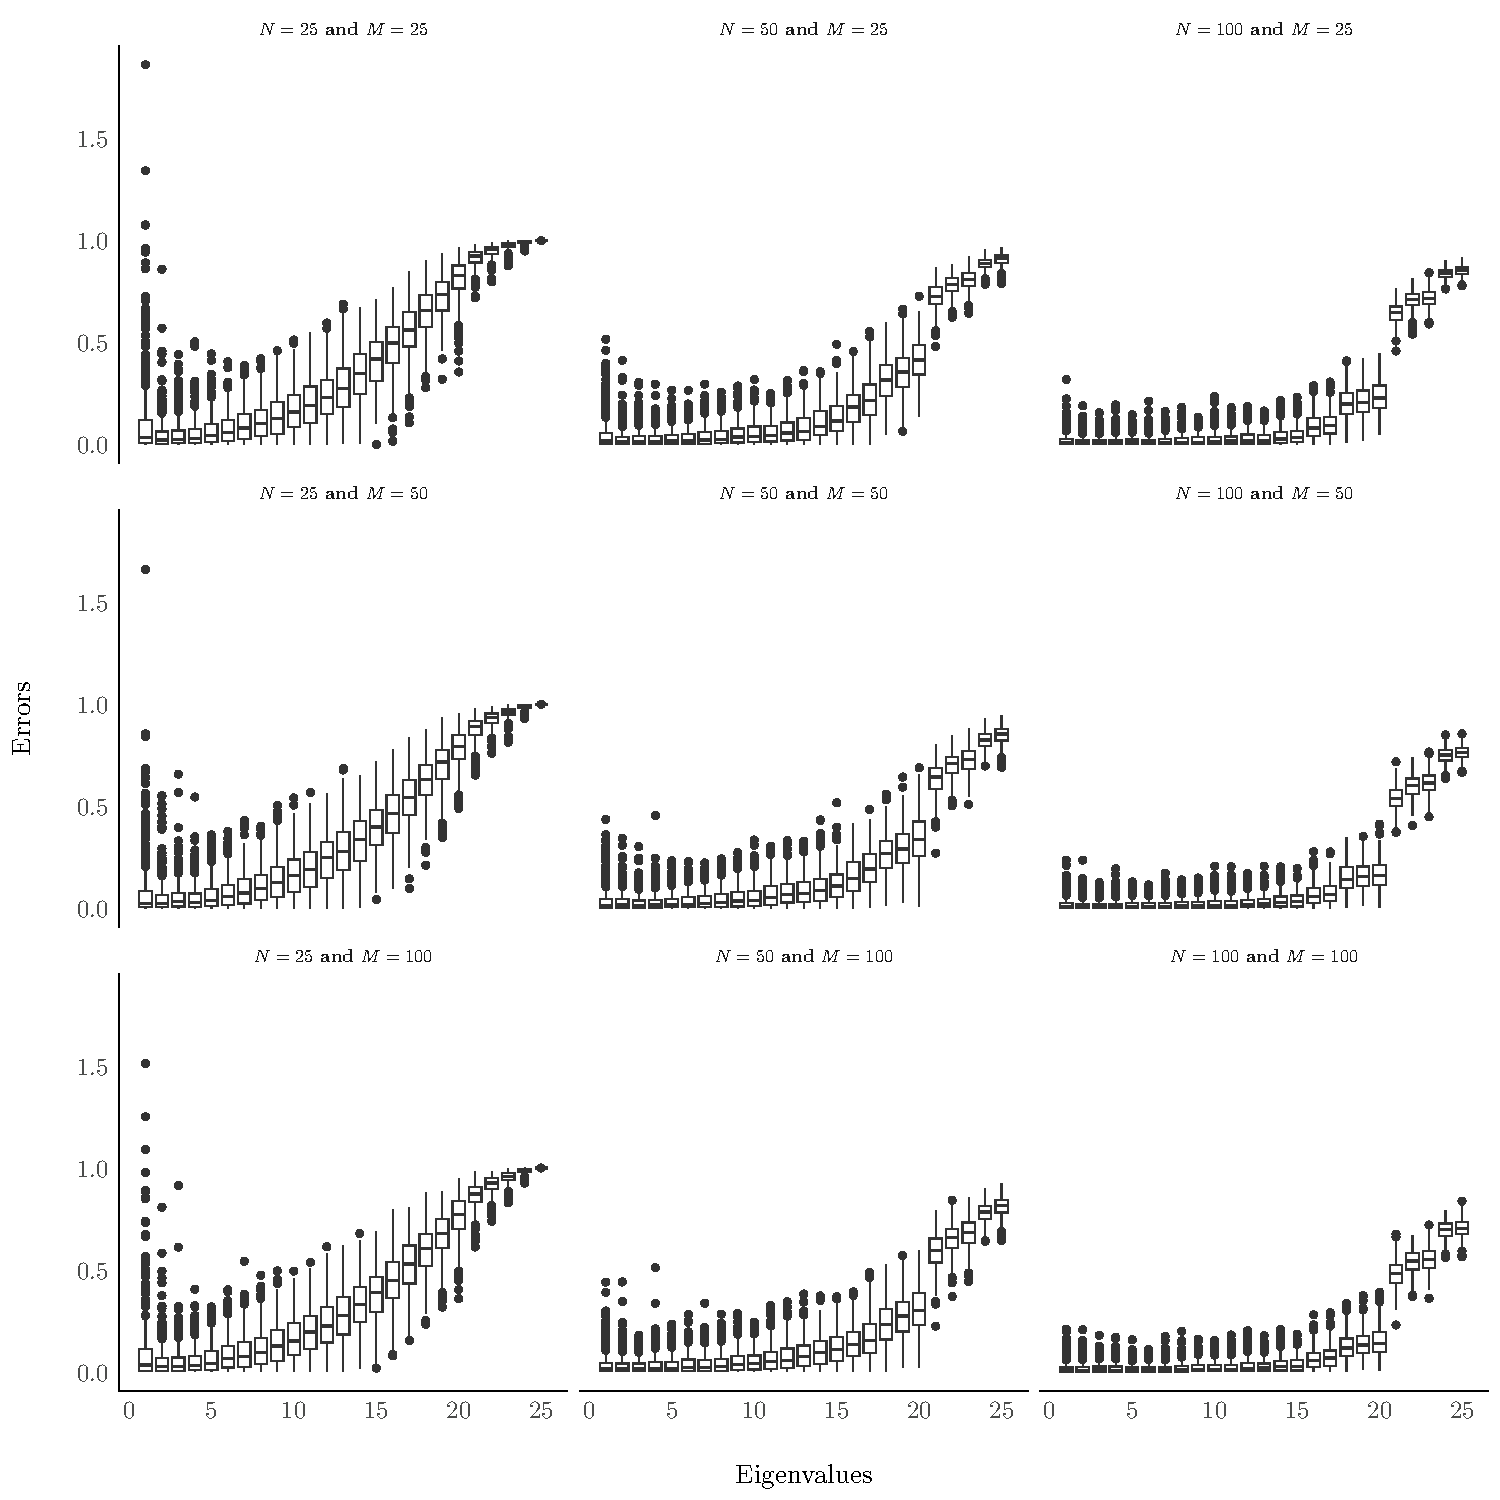
\includegraphics[width=0.95\textwidth]{figures/ncomp.pdf}
    \caption{Boxplots of the estimation errors of the eigenvalues. We estimated $5$ components for each univariate feature. The number of multivariate eigencomponents that can be estimated is thus $25$. $N$ is the number of observations, $M$ is the number of sampling points per curve. We run $500$ simulations.}
    \label{fig:ncomp}
\end{figure}

In Figure \ref{fig:npc_estim}, we present the estimation of the number of components retained for a fix percentage of variance explained over $500$ simulations scenarios. The red dots are the number of components that should be retained for $\alpha\%$ of variance explained, given an exponential decreasing of the eigenvalues as defined in \eqref{eq:npc}. The size of the black dots represents the number of times each components have been selected over the $500$ simulations. We remark that the number of components appears to be underestimated for most combinations of the number of observations $N$, number of sampling points $M$ and percentage of variance explained wanted $\alpha\%$. This results may have an importance for practionners.
\begin{figure}
     \centering
    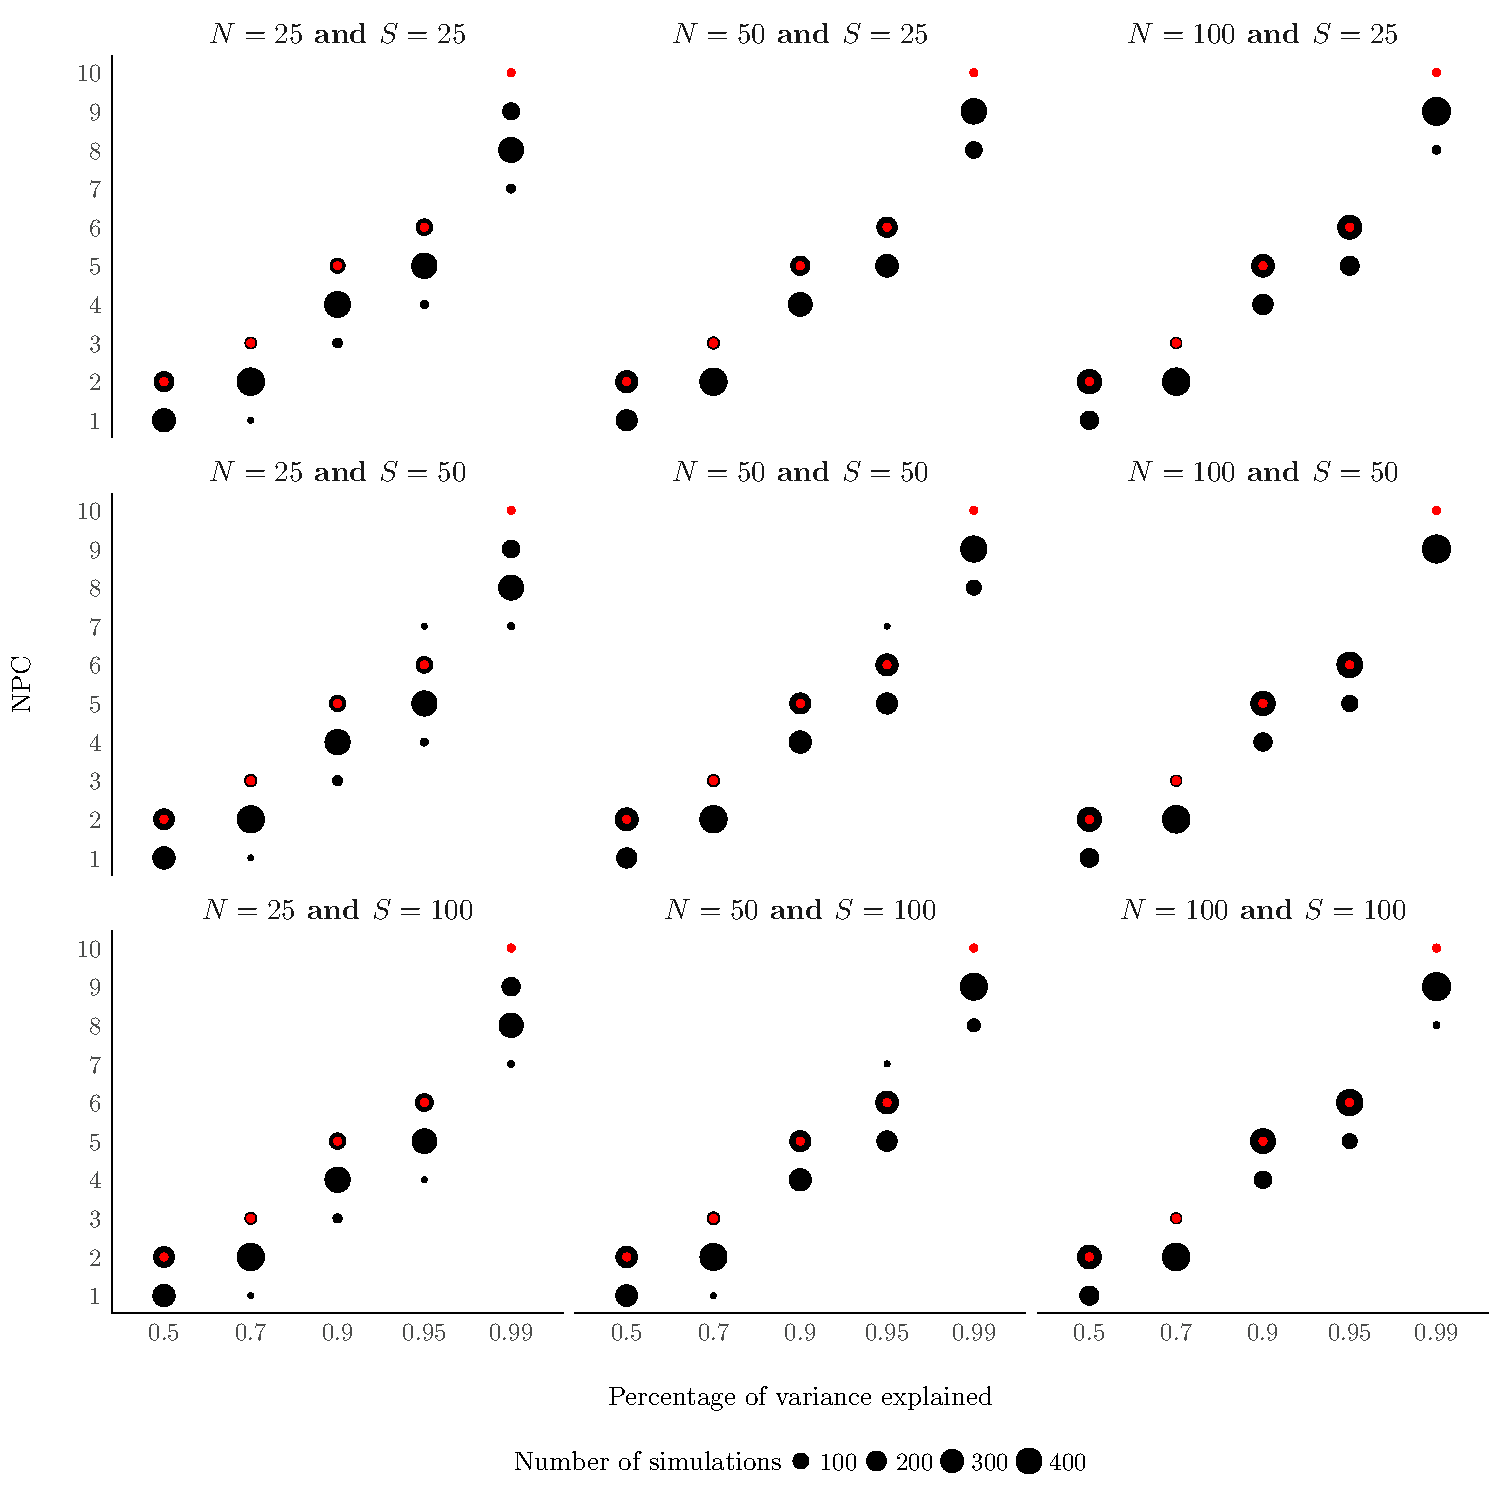
\includegraphics[width=0.95\textwidth]{figures/npc_estim.pdf}
    \caption{The size of the black dots represents the number of times the number of components has been selected over $500$ simulations. The red dots are the true number of components given the percentage of variance explained. $N$ is the number of observations, $M$ is the number of sampling points per curve.}
    \label{fig:npc_estim}
\end{figure}

In Figure \ref{fig:pct_estim}, we present an estimation the percentage of variance explained as the ratio between the sum of estimated eigenvalues and the sum of the true eigenvalues, defined by
\begin{equation}
     \widehat{\text{PVE}}_{1:k} = \frac{\sum_{l = 1}^k \widehat{\nu}_l}{\sum_{l^\prime = 1}^K \nu_{l^\prime}}.
\end{equation}
Due to estimation errors, this quantity can be larger than $1$. For all $\alpha$, except $\alpha = 0.99$, the estimation of the percentage of variance explained is higher than the true percentage of variance explained, which is coherent with the fact that we select the smallest number of components such that at least $\alpha\%$ of the variance is explained by this number of components. For $\alpha = 0.99$, each component explains so little variance by itself that if the number of components is poorly estimated it will not change the percentage of variance explained by the all.
\begin{figure}
     \centering
    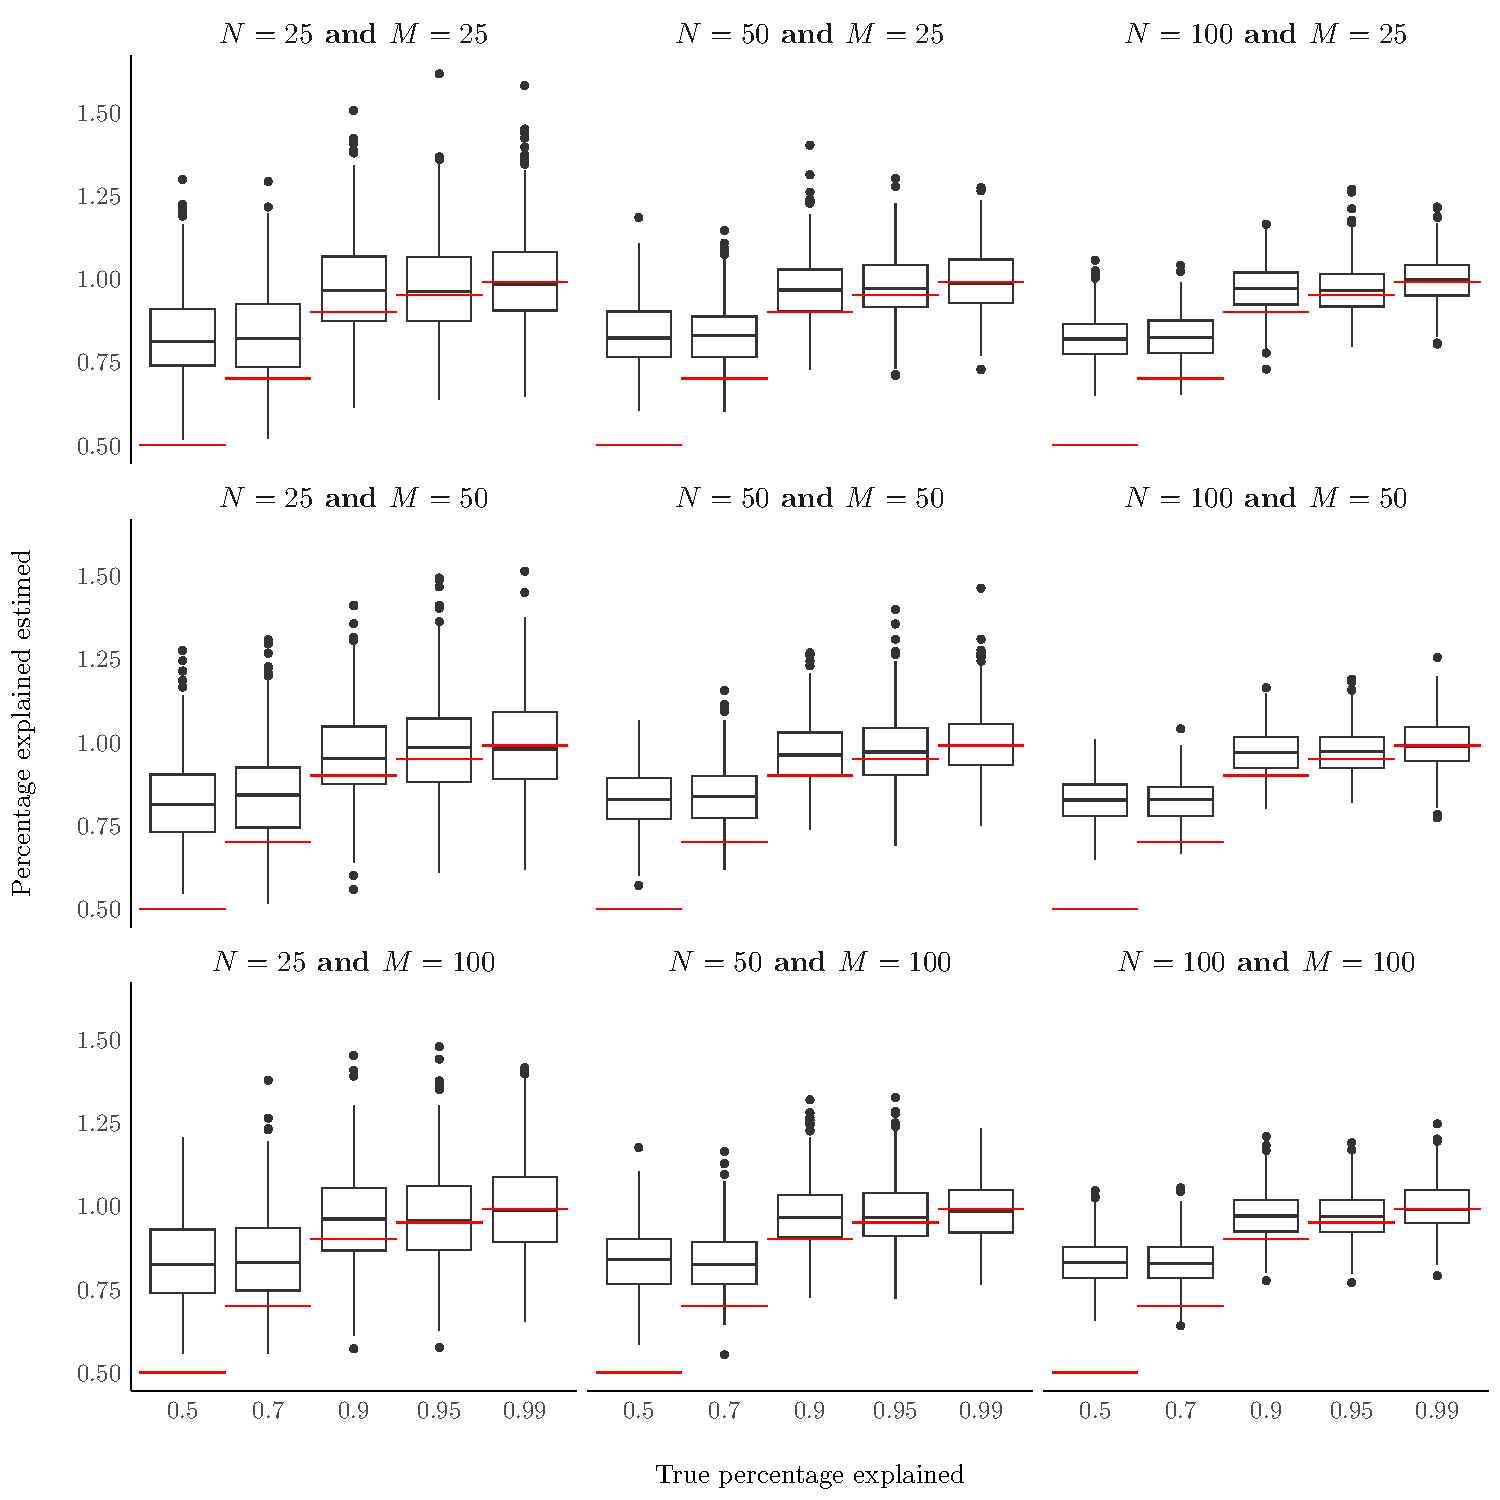
\includegraphics[width=0.95\textwidth]{figures/pct_estim.pdf}
    \caption{Estimation of the percentage of variance explained over $500$ simulations. The red lines are the true percentage of variance explained. $N$ is the number of observations, $M$ is the number of sampling points per curve. The estimation can be larger than $1$ has the estimated cumulative eigenvalues are compare to the true cumulative eigenvalues. We run $500$ simulations.}
    \label{fig:pct_estim}
\end{figure}

To conclude, we would like the practionner to be careful when selecting the number of components for an MFPCA. Keeping all the estimated components from \cite{happMultivariateFunctionalPrincipal2018a} methodology may lead to poorly estimated components and selecting the number of components using the percentage of variance explained may lead to inconsistencies. To solve the first problem, we propose to only use the first $\min_p K_p$ estimated multivariate components. For the second, we recommend doing simulations that mimics the data at hand.
The codes to reproduce the simulations, as well as more results, are available at \url{https://github.com/FAST-ULxNUIG/variance_mfpca}.